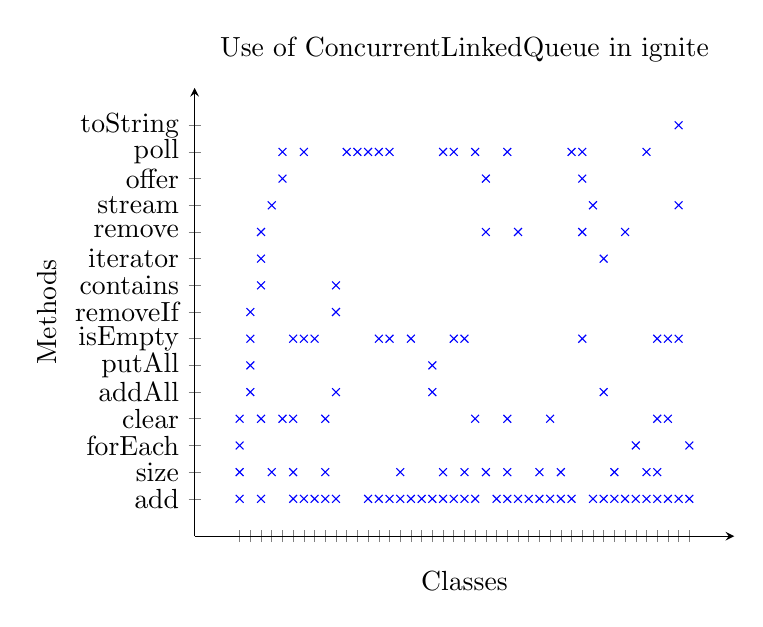
\begin{tikzpicture}
\begin{axis}[scatter/classes={U={mark=+,red}, NU={mark=x,blue}}, legend pos=outer north east,axis x line=bottom, axis y line=left, enlarge x limits=true, xlabel = {Classes}, ylabel = {Methods}, enlarge y limits=true, xtick = data, xticklabels = {,,},ytick=data, yticklabels={add,size,forEach,clear,addAll,putAll,isEmpty,removeIf,contains,iterator,remove,stream,offer,poll,toString}, title={Use of ConcurrentLinkedQueue in ignite}]
\addplot[scatter,only marks, scatter src=explicit symbolic]
coordinates {
(0,0) [NU]
(0,1) [NU]
(0,2) [NU]
(0,3) [NU]
(1,4) [NU]
(1,5) [NU]
(1,6) [NU]
(1,7) [NU]
(2,0) [NU]
(2,8) [NU]
(2,9) [NU]
(2,3) [NU]
(2,10) [NU]
(3,1) [NU]
(3,11) [NU]
(4,12) [NU]
(4,3) [NU]
(4,13) [NU]
(5,0) [NU]
(5,1) [NU]
(5,3) [NU]
(5,6) [NU]
(6,0) [NU]
(6,6) [NU]
(6,13) [NU]
(7,0) [NU]
(7,6) [NU]
(8,0) [NU]
(8,1) [NU]
(8,3) [NU]
(9,0) [NU]
(9,8) [NU]
(9,4) [NU]
(9,7) [NU]
(10,13) [NU]
(11,13) [NU]
(12,0) [NU]
(12,13) [NU]
(13,0) [NU]
(13,6) [NU]
(13,13) [NU]
(14,0) [NU]
(14,6) [NU]
(14,13) [NU]
(15,0) [NU]
(15,1) [NU]
(16,0) [NU]
(16,6) [NU]
(17,0) [NU]
(18,0) [NU]
(18,4) [NU]
(18,5) [NU]
(19,0) [NU]
(19,1) [NU]
(19,13) [NU]
(20,0) [NU]
(20,6) [NU]
(20,13) [NU]
(21,0) [NU]
(21,1) [NU]
(21,6) [NU]
(22,0) [NU]
(22,3) [NU]
(22,13) [NU]
(23,12) [NU]
(23,1) [NU]
(23,10) [NU]
(24,0) [NU]
(25,0) [NU]
(25,1) [NU]
(25,3) [NU]
(25,13) [NU]
(26,0) [NU]
(26,10) [NU]
(27,0) [NU]
(28,0) [NU]
(28,1) [NU]
(29,0) [NU]
(29,3) [NU]
(30,0) [NU]
(30,1) [NU]
(31,0) [NU]
(31,13) [NU]
(32,12) [NU]
(32,6) [NU]
(32,13) [NU]
(32,10) [NU]
(33,0) [NU]
(33,11) [NU]
(34,0) [NU]
(34,9) [NU]
(34,4) [NU]
(35,0) [NU]
(35,1) [NU]
(36,0) [NU]
(36,10) [NU]
(37,0) [NU]
(37,2) [NU]
(38,0) [NU]
(38,1) [NU]
(38,13) [NU]
(39,0) [NU]
(39,1) [NU]
(39,3) [NU]
(39,6) [NU]
(40,0) [NU]
(40,3) [NU]
(40,6) [NU]
(41,0) [NU]
(41,11) [NU]
(41,6) [NU]
(41,14) [NU]
(42,0) [NU]
(42,2) [NU]
};
\end{axis}
\end{tikzpicture}